\hypertarget{2}{}

\chapter{Related Work}

\rhead{Related Work}
\lhead{Chapter 2}

\vspace{-1.6cm}

% Gray Line
\begingroup
\color{gray}
\par\noindent\rule{\textwidth}{0.4pt}
\endgroup

\noindent{This chapter provides an overview of the key concepts to understand Relation Extraction (RE) according to the three main objectives established in Chapter \hyperlink{1}{1}. It also presents some of the initial approaches for RE, by order of complexity \citep{sousa2019using}. Furthermore, it describes the different deep learning methods and how they can be combined in systems for RE, and the steeps needed for their evaluation. Additionally, it introduces semantics for RE, based on knowledge bases and graphs (e.g., ontologies) and semantic similarity metrics. Finally, it characterizes the case study dataset and presents potential challenges with the human phenotype-gene RE.}

% ------------------------------> LEARNING FOR RELATION EXTRACTION

\section{Learning for Relation Extraction}

Using different sources of information to support automated extracting of relations between biomedical concepts contributes to the development of our understanding of biological systems. Researchers have proposed several RE approaches to identify relations between concepts in biomedical literature, namely, using neural network algorithms. The use of multichannel architectures composed of multiple data representations, as in deep neural networks, leads to state-of-the-art results. The right combination of data representations can eventually lead us to even higher evaluation scores in RE tasks. The following sections will present the baseline concepts that are the building blocks for RE, the initial approaches to perform RE, and the different approaches, systems, and evaluation tools for deep learning RE.  

% ------------------------------> NATURAL LANGUAGE PROCESSING

\hypertarget{2.1.1}{\subsection{Natural Language Processing}}

Natural Language Processing (NLP) is a field in computer science that aspires to obtain meaning from highly heterogeneous or unstructured text written by humans. This field covers several techniques that constitute pre-processing steps for the tasks described in the following section. NLP techniques target different goals and are often combined to obtain higher performance. 

\textbf{Tokenization} breaks the text into tokens to be processed individually or as a sequence. The tokens are usually words but can also be phrases, numbers, and other types of elements. 
The most straightforward form of tokenization is breaking the input text by whitespaces or punctuation. However, with literature that is descriptive and formal, we have to account for complex entities. These entities tend to be morphological complex and need specialized tokenization pipelines. Some researchers use a compression algorithm \citep{sennrich2015neural}, byte pair encoding (BPE), to account for vocabulary variability. BPE represents open vocabularies through a fixed-size vocabulary of variable-length character sequences, making it suitable for neural networks models, for instance.

\textbf{Stemming and Lemmatization} reduces the variability of natural language by normalizing a token to its base form (stem) \citep{manning2008introduction}. Also, it can take into account the context of the token, along with vocabulary and morphological analysis to establish the canonical form of the word (lemma). The lemma is always a real word, but the stem can correspond only to a fragment of a word. For example, the stem of the word \textit{having} is \textit{hav}, and the lemma is \textit{have}.
    
\textbf{Part-of-Speech Tagging} assigns each word of a sentence to the category where it belongs, taking into account their context (e.g., adverb or preposition). Each word can belong to one or more categories. This feature expresses the role of a word in a given sentence. 
    
\textbf{Parse Tree} represents the syntactic structure of a sentence. There are two different types of parse trees: constituency-based parse trees and dependency-based parse trees. The main difference between the two is the distinction between the terminal and non-terminal nodes. The first makes that distinction, and in the second, all nodes are terminal. In constituency-based parse trees, each node of the tree is either a \textit{branch} node, a \textit{leaf} node, or a \textit{root} node. For each sentence, there is only one \textit{root} node. The \textit{leaf} node is terminal, and the \textit{branch} node connects to two or more \textit{child} nodes. These leaves correspond to the lexical tokens \citep{aho1986compilers}. 
Dependency-based parse trees are usually simpler because they only identify the primary syntactic structure, leading to fewer nodes. 
The structures created by parse trees are used as inputs for other algorithms and can be constructed based on supervised learning techniques.

% ------------------------------> TEXT MINING

\hypertarget{2.1.2}{\subsection{Text Mining Primary Tasks}}

Text mining has become a widespread approach to identify and extract information from unstructured or highly heterogeneous text \citep{westergaard2018comprehensive}. Text mining is used to extract facts and relationships in a structured form that can be used to annotate specialized databases and transfer knowledge between domains \citep{fleuren2015application}. Text mining can be considered as a sub-field of data mining. Thus, with the transformation of text into proper data representations, we can apply data mining algorithms, namely numeric vectors. In recent years, text mining tools have evolved remarkably in quality and number, but there are still several challenges in applying text mining to scientific literature. The main challenges are the heterogeneity and complexity of the written resources, making the retrieval of relevant information (i.e., relations between entities) a non-trivial task. 

Text Mining tools can target different tasks separately or together. Some of the primary tasks are Named Entity Recognition (NER), Named-Entity Linking (NEL), and RE. 

\textbf{Named Entity Recognition (NER)} seeks to recognize and classify entities mentioned in the text by identifying the offset of its first and last character. This task's workflow starts by splitting the text in tokens and then labelling them into categories (part-of-speech (POS) tagging).
    
\textbf{Named-Entity Linking (NEL)} maps the recognized entities (in the previous step) to entries in a given knowledge base. For instance, an entity can be written in various ways and mentioned by different names or acronyms in a text. NEL links all these distinct nomenclatures to one unique identifier. 
    
\textbf{Relation Extraction (RE)} identifies relations between entities (recognized by NER or manually) in a text. Tools mostly consider relations by the co-occurrence of the entities in the same sentence. However, some progress is being made to extend this task to the full document (taking into account a global context) \citep{singhal2016text}.

% ------------------------------> INITIAL APPROACHES FOR RELATION EXTRACTION

\subsection{Initial Approaches for Relation Extraction}

Through the years, RE dedicated approaches are becoming increasingly more intricate with the associated growth in performance. This section describes the RE approaches and some of their applications, that preceded the deep learning-based RE systems. Due to the inherent complexity of highly heterogeneous or unstructured literature, initial approaches for RE worked on a sentence level \citep{lamurias2017extracting} and focused primarily on binary relations \citep{zhang2017review}.


\subsubsection{Co-occurrence}

Co-occurrence assumes that if two entities are mentioned in the same sentence (co-occur), they are likely related. Usually, this approach's application results in a higher recall (most of the entities co-occurring in a sentence participate in a relation) and lower precision. 
Some methods use frequency-based scoring schemes to eliminate relations identified by chance \citep{zweigenbaum2007frontiers}. Nowadays, most applications use co-occurrence as a baseline against more complex approaches \citep{bunescu2006integrating}. 


\hypertarget{2.1.3.2}{\subsubsection{Pattern-based}}

Pattern-based uses manually defined patterns and automatically generated patterns to extract relations.

\textbf{Manually defined patterns} require domain expertise knowledge about the type of entities, their interactions, and the text subject at hand. 
Initial systems made use of regular expressions to match word patterns that reflected a relation between two entities \citep{smolinski2009computational}, making use of a dictionary of words that express relation, such as \textit{trigger} and \textit{stimulate}. Later systems introduce part-of-speech (POS) tagging, but this has proven to be too naive, mainly when applied to complex sentences, such as the ones that we typically find in scientific literature \citep{hao2005discovering}. Opposite to the co-occurrence approaches, manually defined patterns frequently achieve high precision but tend to have poor recall. This approach does not generalize well, and therefore is difficult to apply to new unseen data. 

\textbf{Automatically generated patterns} encompass two main approaches, bootstrapping with seeds \citep{wang2011inference} and leveraging of the corpora \citep{liu2011graphs}. 
The bootstrapping method uses a small set of relations known as seeds (e.g., person-occupation pairs). The first step is to identify the seeds in the dataset and map the relation pattern they describe. The second step is to try to apply the mapped patterns to the dataset to identify new pairs of relations that follow the same construction. Finally, the original set of relations is expanded by adding these new pairs. When, after repeating all previous steps, no more pairs are found, the process ends. Some systems apply distant supervision techniques to keep track of the validity of the added patterns. Distant supervision uses existing knowledge base entries as gold standards to confirm or discard a relation \citep{jiang2018revisiting}. This method is susceptible to noisy patterns, as the original set of relations grows.
On the other hand, the leveraging of the corpora method makes immediate use of the entire dataset to generate the patterns. This method requires a higher number of annotated relations and produces highly specific patterns that cannot match new unseen data. Automatically generated patterns can achieve higher recall than manually defined patterns, but overall the noisy patterns continue to damage the precision. Nevertheless, there are a few efforts to reduce the number of noisy patterns \citep{nguyen2010simple}. 


\subsubsection{Rule-based}

Rule-based also uses manually defined and automatically generated rules from the training data to extract relations. Depending on the systems, the differences between pattern-based and rule-based approaches can be minor. 
Ruled-based approaches not only use patterns but also additional restraints to cover issues that are difficult to express by patterns, such as checking for the negation of the relations \citep{koike2005automatic}. Some ruled-based systems distance themselves from pattern-based approaches by replacing regular expressions with heuristic algorithms and sets of procedures \citep{rinaldi2007mining}. Like pattern-based approaches, ruled-based approaches tend to have poor recall, even though rules tend to be more flexible. The trade-off recall/precision can be improved using automatic methods for rule creation \citep{xu2012feature}.


\subsubsection{Machine Learning (ML)-based}

Accordingly to the types of corpora, researchers divide RE based on machine learning into three domains \citep{zhang2017review}: supervised learning methods, semi-supervised learning methods, and unsupervised learning methods, beyond the deep learning methods described in Section \hyperlink{2.4}{2.4}. 

\textbf{Supervised machine learning }makes use of large annotated corpora to perform RE. These corpora are pre-processed using NLP tools and then used to train classification models. Beyond deep learning, described in detail in Section \hyperlink{2.1.4}{2.1.4}, it is possible to categorize these ML methods into two main approaches, Feature-based and Kernel-based. \textbf{Feature-based approaches} represent each instance (e.g., a sentence) as a vector in an $n$-dimensional space. Support Vector Machines (SVM) classifiers tend to be used to solve binary classification problems and are considered black-boxes because there is no user interference in the classification process. These classifiers can use different features that are meant to represent the data characteristics (e.g., shortest path, bag-of-words (BOW), and POS tagging) \citep{kim2008detection}. \textbf{Kernel-based approaches} main idea is to quantify the similarity between the different instances in a dataset by computing the similarities of their representations \citep{giuliano2006exploiting}. Kernel-based approaches add the structural representation of instances (e.g., by using parse trees). These methods can use one kernel or a combination of kernels (e.g., graph, sub-tree (ST), and shallow linguistic (SL)). SVM classifiers do not need to use kernels. However, kernels are commonly used in these classifiers, to the point where its use is subtended by most users. 

\textbf{Semi-supervised or weekly supervised learning} methods mainly encompass the bootstrap method described previously (Section \hyperlink{2.1.3.2}{2.1.3.2}) \citep{hoffmann2011knowledge,augenstein2015extracting}. It is mostly used in the field of knowledge extraction to solve classification and relation extraction problems. 
This learning method reduces the dependence of human participation and corpus annotation. However, the bootstrap method has the problem of semantic drift when in the iterative process, damaging the RE's performance.

Supervised and semi-supervised learning methods need to determine the type of relation in advance. Large-scale corpora implies multiple relations, and, most of the time, those methods are not able to grasp all of that variety. Therefore, researchers started using \textbf{unsupervised learning} based on the idea of clustering \citep{hasegawa2004discovering,shinyama2006preemptive}. 
The idea was to use text information clustering between two entities to express the relation class. This formulation was successfully applied to multiple approaches and improved to multilevel clustering by \cite{shinyama2006preemptive}. In unsupervised learning, some researchers also developed methods based on pattern clustering (i.e., Density-based methods) and sentence parsing \citep{quan2014unsupervised}. 
This category of methods makes it hard to describe the relation name accurately and has difficulties catching low-frequency relations (low recall).

% ------------------------------> DEEP LEARNING FOR RELATION EXTRACTION

\hypertarget{2.1.4}{\subsection{Deep Learning for Relation Extraction}}

Artificial neural networks are a parallel combination of small processing units (nodes) which can acquire knowledge from the environment through a learning process and store the knowledge in the connections between the nodes \citep{haykin1994neural} (represented by direct graphs \citep{guresen2011definition}). The process is inspired by the biological brain function, having each node corresponding to a \textit{neuron} and the connections between the nodes representing the \textit{synapses}. Artificial neural networks use fully connected layers to connect every neuron in one layer to every neuron in another layer. 
The first application of neural networks to NLP was language modelling, which has been useful to learn distributed representations (embeddings) for words \citep{bengio2003neural,mikolov2013distributed}. These data representations (i.e., word embeddings) were the initial step for a new way to successfully perform several NLP tasks, based on neural networks \citep{nguyen2015relation}.  


\subsubsection{Convolutional Neural Networks (CNN)}

Deep learning RE systems use Convolutional Neural Networks (CNN) to further encode the sentences, capturing $n$-gram level features. CNN consists of three parts: the input layer; the output layer; and several hidden layers, including convolutional layers, pooling layers, fully connected layers, and normalization layers \citep{xue2018relation}. 
In the convolutional layers, a convolution operation reduces the number of free parameters in the following way. Given an input sentence $x$ as a sequence of vectors $x = \{w_1,w_2,...,w_m\},\ w_i \in \mathbb{R}^d$, where $w_i$ represents the words in the $x$ sentence,  $m$ is the size of the input sentence, and $d$ is the dimensionality of the embedding space. If we have $l$ as the window size for the convolutional layer kernel, then the vector for the $i$-th window is formed by concatenating the input vectors for that window:

\begin{equation}
    q_i = w_{i:i+l-1};\ (1 \leq i \leq m-l+1);\ q_i \in \mathbb{R}^{(d \times l)}
\end{equation}

Then, a single convolutional kernel could be represented by a weight vector $W$ and a bias $b$, and the output for the $i$-th window computed as:

\begin{equation}
    p_i= f (W'q_i+b)
\end{equation}

where $f$ is the activation function. The shape of the output of the convolutional kernel $p$ would be $p \in \mathbb{R} ^{(m-l+1)}$. If the convolutional layer was a set of $d_c$ convolutional kernels, the output of the layer would be of the shape $\mathbb{R} ^{d_c \times (m-l+1)}$.
The convolutional operation allows the network to be more in-depth with fewer parameters, passing the result to the pooling layers. These layers (and also convolutional layers) provide a fixed size output matrix and reduce the output dimensionality while keeping the essential information. 

\hypertarget{2.1.4.2}{\subsubsection{Recurrent Neural Networks (RNN)}}

Recurrent Neural Networks (RNN) is a type of artificial neural network where the nodes' connections follow a contrary path to the flux of data. Thus, RNN can use their internal state, or \textit{memory}, to process each input sequence. 
Deep learning techniques, such as RNN, aim to train classification models based on word embeddings, part-of-speech (POS) tagging, and other features. RNN classifiers have multilayer architectures, where each layer learns a different representation of the input data. This characteristic makes RNN classifiers flexible to multiple text mining tasks, without requiring task-specific feature engineering. Hence, while training, RNN keep remembering the context, and each state can be defined by:

\begin{equation}
    h_t = f(h_{t-1}, x_t)
\end{equation}

where $x_t$ refers to the input and $h_t$ symbolizes the output, at a given time ($t$). Then, to each state we apply an activation function:

\begin{equation}
    h_t = tanh(W_{hh} \times h_{t-1} + W_xh \times x_t)
\end{equation}

where $W$ is the weight, $h$ is the single hidden vector, $Whh$ is the weight at the previous hidden state, $Whx$ is the weight at the current input state, and $tanh$ is the activation function that implements a non-linearity that squashes the activations to the range $[-1,1]$. Then, the output state is:

\begin{equation}
    y_t = W_{hy} \times h_{t}
\end{equation}

where $Why$ is the weight at the output state.

\paragraph{Long Short-Term Memory Networks (LSTMs)}

Long Short-Term Memory (LSTM) networks are an alternative to regular RNN \citep{hochreiter1997long}. LSTMs are a type of RNN that handles long dependencies (e.g., sentences), making this classifier more suitable for scientific domains, for instance, where sentences are usually long and descriptive. LSTMs solve the vanishing problem of RNN, using back-propagation, and its main constituents are three gates (the input gate, the output gate, and the forget gate).
In recent years, the use of LSTMs to perform RE tasks has become widespread in various domains, such as semantic relations between nominals \citep{miwa2016end}. \textbf{Bidirectional LSTMs} use two LSTM layers, at each step, one that reads the sentence from right to left, and other that reads from left to right. The combined output of both layers produces a final score for each step. Bidirectional LSTMs have yield better results than traditional LSTMs when applied to the same datasets \citep{zhang2015bidirectional}.

\hypertarget{2.1.4.3}{\subsubsection{Data Representations}}

The combination of multiple and different language and entity related data representations is vital for the success of neural network models dedicated to RE tasks. Some of these features were already described in Section \hyperlink{2.1}{2.1}, such as POS tagging and parse trees. 

\textbf{Shortest Dependency Path} (SDP) is a feature that identifies the words between two entities mentioned in the text, concentrating the most relevant information while decreasing noise \citep{xu2015classifying}. 

\textbf{Word Embeddings} are fixed-sized numerical vectors that aim to capture the syntactic and semantic word relationships. These word vectors models use multiple different pre-training sources. For instance, Word2Vec \citep{mikolov2013distributed} uses English Wikipedia, and BERT \citep{devlin2019bert} uses both English Wikipedia and BooksCorpus. 
Early models, such as Word2Vec, learned one representation per word, but this proved to be problematic due to polysemous and homonymous words. Recently, most systems started to apply one embedding per word sense. One of the reasons why BERT outperforms previous methods is because it uses contextual models, meaning that it generates a unique representation for each word in a sentence. For instance, in the sentence fragments, \textit{they got \textbf{engaged}}, and \textit{students were very \textbf{engaged} in}, the word \textit{engaged} for non-contextual models would have the same meaning. BERT also outperforms other word vector models that take into account the sentence context, such as ELMo \citep{peters2018deep} and ULMFit \citep{howard2018universal}, due to being an unsupervised and deeply bidirectional pre-trained language representation.

\textbf{WordNet Hypernyms} are a feature that helps to hierarchize entities, structuring words similar to direct acyclic graphs \citep{miller1998wordnet}. For example, a \textit{vegetable} is a hypernym of \textit{tubers}, which in turn constitutes a hyponym of \textit{vegetable}. This feature is comparable to an ontology in the sense that a hierarchy relation is identified, but misses the identification of relations between the different terms.

Using different features as information sources feeding individual channels leads to multichannel architecture models. Multichannel approaches were proven to be effective in RE tasks \citep{xu2015classifying}. 

Regarding biomedical RE, LSTMs were successful in identifying drug-drug interactions \citep{wang2017dependency}, gene-mutation relations \citep{song2018n}, drug-mutation relations \citep{peng2017cross}, among others. Some methods use domain-specific biomedical resources to train features for biomedical tasks. BioBERT \citep{lee2020biobert} is a domain-specific language representation model pre-trained on large-scale biomedical corpora, based on BERT \citep{devlin2019bert} architecture. BioBERT, using minimal task-specific architecture modifications, significantly outperforms previous biomedical state-of-the-art models in the text mining primary tasks of Named-Entity Recognition, Named-Entity Linking, and RE. The BR-LSTM \citep{xu2018leveraging} model uses a multichannel approach with pre-trained medical concept embeddings. Using the Unified Medical Language System (UMLS) concepts, BR-LSTM applies a medical concept embedding method developed by \cite{de2014medical}. BO-LSTM \citep{lamurias2019bo} uses the relations provided by domain-specific ontologies to aid the identification and classification of relations between biomedical entities in biomedical literature. 

\hypertarget{2.4.4}{\subsubsection{Systems}}

Models created by existing state-of-the-art deep learning RE systems aim to learn useful entities and relations features from a given sentence. These systems do not need complicated feature engineering, but they tackle tasks differently, yielding different results. There are two main sub-sets of models: pipeline models and joint models. 

\paragraph{Pipeline Systems}

In pipeline models, the tasks are divided into the NER and RE parts. The pipeline models are based on the following deep neural networks:

\begin{itemize}
    \item \textbf{CNN} preserve sequence information and extract the keyword information in a sentence, exhibiting state-of-the-art results on the semantic representations of sentences. 
    \item \textbf{LSTMs and Bidirectional LSTMs} capture long-range dependencies of sequences, extracting syntactical information of sentences, and, therefore, are suited for text analysis. 
\end{itemize}

\paragraph{Joint Systems}

Joint models allow us to learn related features from a given sentence and make full use of the sub-tasks. Some joint model proposals are:

\begin{itemize}
    \item \cite{li2014incremental} built a model that incrementally predicts entities and relations using a single joint model (End-to-end 1 (Table \ref{tab2})).
    \item \cite{miwa2016end} capture both word sequence and dependency tree substructure information by stacking bidirectional tree-structured LSTM-RNNs on bidirectional sequential LSTM-RNN (End-to-end 2 (Table \ref{tab2})).
    \item \cite{li2016joint} use a CNN to represent variable-length features such as multi-word entity mentions and leverage of rectified linear units (RELU) in the hidden layer while using a cube activation function (Joint 1 (Table \ref{tab2})).
    \item \cite{li2017neural} used parameter sharing between two Bi-LSTM-RNN networks (Joint 2 (Table \ref{tab2})).
\end{itemize}


% ------------------------------> EVALUATION OF DEEP LEARNING SYSTEMS

\subsubsection{Evaluation Metrics for RE}

The evaluation of deep learning systems is done by applying the trained models to a gold standard test-set. They are manually curated or annotated by domain experts and unseen by the system. For a RE task, the gold standard test-set should correspond to the list of pairs of entities (e.g., person-organization or gene-disease pairs) that co-occur in the same sentences and their relation.

To any given information extraction system, it is necessary to define what constitutes a positive and negative result, particularly in the biomedical domain. Researchers and clinicians need to have access not only to known relations between biomedical entities but also to relations that were already disproven \citep{sousa2020improving}. Accessible negative results limit their search space and prevent the costly re-exploration of research hypotheses. However, most biomedical relation extraction datasets do not seek to distinguish between a false and a negative relation among two biomedical entities, and few knowledge bases hold negative examples. Some domain-specific exceptions are worth noticing, such as the Negatome database \citep{blohm2014negatome} for protein-protein interactions, and the phenotype-disease relations annotation file made available by the Human Phenotype Ontology (HPO) organization \citep{robinson2010human} that contains both positive and negative relations.

A false relation should express a context where the entities are not related. In contrast, a negative relation should express a context where there is an affirmation of no association between the two entities. Furthermore, datasets created using distant supervision techniques also have some false negative relations that constitute undocumented/unknown relations \citep{sousa2019silver}. These relations are not marked true because they are not described in a knowledge base at the moment of the dataset creation, even though upon reading the context of these relations within their respective sentences one can support a true relation. Unknown relations are good examples of hypotheses to be further explored by researchers and clinicians and can be of use to effectively populate the biomedical relations knowledge bases. In RE tasks, the binary type of results possible are Relation that can be either positive or negative, and No Relation that is only false, shown in Table \ref{table:evaluation}.

\begin{table}[ht]
\renewcommand\arraystretch{1.2}
\centering
\caption[Types of Results Obtained with an Information Extraction System for a RE Task]{Types of results obtained with an information extraction system for a RE task.}
\begin{tabular}{ |c|c|c| }
\hline
\textbf{Annotator (Gold Standard)} & \textbf{System} & \textbf{Classification}\\
\Xhline{2\arrayrulewidth}
\multirow{2}{*}{Relation} & Relation & True Positive (TP) \\
\cline{2-3}
 & No Relation & False Negative (FN) \\ 
\hline
\multirow{2}{*}{No Relation} & Relation & False Positive (FP) \\
\cline{2-3}
 & No Relation & True Negative (TN) \\
 \hline
\end{tabular}
\label{table:evaluation}
\end{table}

The primary goal of a given information retrieval system is to maximize the number of TP and TN. To compare results obtained with different datasets or different tools, we have three distinct evaluation metrics: recall, precision, and F-measure. Precision represents how often the results are correct, recall the number of correct results identified, and F-measure is a combination of both metrics to express overall performance, being the harmonic mean of precision and recall:

\begin{equation}
F-measure = \frac{2\times Precision\times Recall}{Precision + Recall} = \frac{2 TP}{2 TP + FP + FN}
\label{equation:evaluation}
\end{equation} 


\subsection{Datasets}

There are three types of datasets for RE. The first type is the \textbf{traditional information extraction datasets}, where relations are manually annotated and pre-determined. Some examples of these type of datasets:

\begin{itemize}
    \item \textbf{AImed} \citep{mooney2006subsequence} describes interactions between human proteins.
    \item \textbf{SemEval 2007} \citep{girju2007semeval} and \textbf{SemEval 2010} \citep{hendrickx2010semeval} describe relations between nominals.
    \item \textbf{Wikipedia} \citep{culotta2006integrating} describes relations person-to-person, and between people and organizations. 
    \item \textbf{Web} \citep{bunescu2007learning} describes person-birthplace relations.
    \item \textbf{BioNLP Shared Task} \citep{kim2011overview} describes relations between proteins and components, and sub-units and complexes. 
    \item \textbf{ADE-V2} \citep{gurulingappa2012development} describes relations between drugs and drug-related adverse effects. 
    \item \textbf{KBP-37} \citep{zhang2015relation} describes relations between bosses and employees. 
\end{itemize}

The second type is \textbf{open information extraction datasets}, where relations are manually annotated but can be of any type. Some examples of these type of datasets:

\begin{itemize}
    \item \textbf{ReVerb} \citep{fader2011identifying} from Yahoo's random link service.
    \item \textbf{ClausIE} \citep{del2013clausie} from Yahoo's random link service and Wikipedia.
    \item \textbf{WEB-500}, \textbf{NYT-500}, and \textbf{PENN-100} \citep{mesquita2013effectiveness} from Wikepedia, the New Your Times, and the Penn Treebank. 
\end{itemize}


Finally, the third type is \textbf{distantly supervised datasets}, where distant supervision is applied, and the relations are usually pre-determined. This last type has been in rapid expansion for being less costly and time-consuming than the previous. Some examples of these type of datasets:

\begin{itemize}
    \item \textbf{ACE 2005 Dataset}\footnote{\url{https://pdfs.semanticscholar.org/3a9b/136ca1ab91592df36f148ef16095f74d009e.pdf}} describes six types of relations: person-social, agent-artifact, GPE-affiliation, part-whole, physical location-physical location, and employment-organization. 
    \item \textbf{NYT Dataset} \citep{riedel2010modeling} describes relations between companies and founders. 
    \item \textbf{Google's relation-extraction-corpus}\footnote{\url{https://github.com/google-research-datasets/relation-extraction-corpus}} describes relations between subjects and objects. 
    \item \textbf{PGR Corpus} \citep{sousa2019silver} describes relations between human phenotypes and genes. 
\end{itemize}

\subsection{Evaluation of System Architectures}

To evaluate the different system architectures described in Section \hyperlink{2.4.4}{2.4.4}, \cite{xue2018relation} used the ACE 2005 Dataset obtaining the results described in Table \ref{tab2}. 

Regarding pipeline systems, systems that involve only CNN-based models are superior to systems that only resort to LSTM-based models. CNN-based models focus on extracting keyword information, while LSTM-based models are focused on representing the sentences’ syntactical information. From Table \ref{tab2}, we can deduct that a mixture of CNN and LSTM contributes to about 10\% improvement in precision and yields a better performance overall.

\begin{table}[H]
\renewcommand\arraystretch{1.3}
\centering
\caption[Results for Different RE Systems Architectures]{Comparison of the results on the ACE 2005 Dataset for different RE systems architectures. Above the double line are the pipeline systems, and below the joint systems. The table is adapted from \cite{xue2018relation}.}\label{tab2}
\newcolumntype{C}{ >{\centering\arraybackslash} m{6cm} }
\newcolumntype{A}{ >{\centering\arraybackslash} m{1.7cm} }
\newcolumntype{B}{ >{\centering\arraybackslash} m{1.5cm} }
\begin{tabular}{|C|B|B|A|}
\hline
\multirow{2}{*}{\textbf{Architectures}} & \multicolumn{3}{c|}{\textbf{Relation Extraction}} \\
\cline{2-4}
& \textbf{Precision} & \textbf{Recall} & \textbf{F-measure} \\
\Xhline{2\arrayrulewidth}
CNN & 0.543 & 0.456 & 0.492 \\
\hline
Bi-LSTM & 0.526 & 0.459 & 0.484 \\
\hline
CNN + LSTM & 0.655 & 0.416 & 0.509 \\
\hline
CNN + CNN & 0.600 & 0.484 & 0.536 \\
\hline
LSTM + LSTM & 0.682 & 0.320 & 0.436  \\
\hline\hline
End-to-end 1 \citep{li2014incremental} & 0.654 & 0.398 & 0.495 \\
\hline
End-to-end 2 \citep{miwa2016end} & 0.572 & 0.540 & 0.556 \\
\hline
Joint 1 \citep{li2016joint} & 0.640 & 0.629 & 0.634 \\
\hline
Joint 2 \citep{li2017neural} & 0.675 & 0.758 & 0.714 \\
\hline
\end{tabular}
\end{table}


The joint models are far superior in performance compared with the pipeline models, with an around 20\% improvement in F-measure. The performance is due to the effective parameter sharing between sub-tasks that helps the joint model capture their interactions.

% ------------------------------> SEMANTICS FOR RELATION EXTRACTION

\hypertarget{2.2}{\section{Semantics for Relation Extraction}} 

Semantic resources such as knowledge bases and graphs can contain highly structured background data, particularly for the biomedical domain \citep{li2020bio}. These resources play a fundamental role in the way we store, organize and retrieve information. More specifically, biological knowledge bases are commonplace for researchers and clinicians to access all types of biomedical data retrieved from biomedical literature \citep{arnaboldi2020text}. These resources can be explored by researchers regarding information retrieval systems, so one can rely on more than the literature itself to train a RE model. By integrating semantic resources, we are feeding the training process with extra, highly relevant information about each entity in the relation and the connections that that entity establishes within the known semantic universe.

% ------------------------------> KNOWLEDGE GRAPHS

\subsection{Knowledge Graphs}

Different perspectives or taxonomies \citep{lee2019attention} can classify graph-structured data. One of those taxonomies that focus on problem setting regarding the type of input relevant for RE is whether the graph is homogeneous or heterogeneous. A homogeneous graph is a graph where all the edges and nodes are of the same type. In contrast, heterogeneous graphs have a set of node types and a set of edge types. A bipartite graph is a simple heterogeneous graph with two node types and a single edge type. Figure \ref{figure:graphs} represents the three types of graphs: \ref{figure:a} homogeneous, \ref{figure:b} heterogeneous, and \ref{figure:c} bipartite graph. 

\begin{figure}
\captionsetup{font=small}
\centering
\begin{subfigure}[b]{0.3\textwidth}
    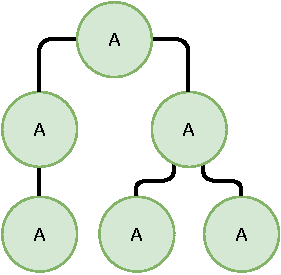
\includegraphics[width=4.5cm]{images/graph_a.pdf}
    \caption{}
    \label{figure:a}
  \end{subfigure}
  \begin{subfigure}[b]{0.3\textwidth}
    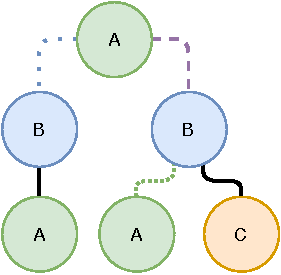
\includegraphics[width=4.5cm]{images/graph_b.pdf}
    \caption{}
    \label{figure:b}
  \end{subfigure}
  \begin{subfigure}[b]{0.3\textwidth}
    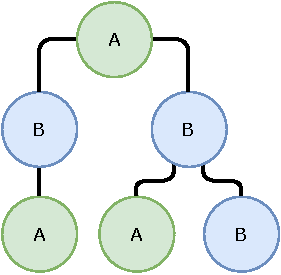
\includegraphics[width=4.5cm]{images/graph_c.pdf}
    \caption{}
    \label{figure:c}
  \end{subfigure}
\fontsize{9}{10.8}\caption[Types of Graphs According to Input]{Three types of graphs, according to type of input: \textbf{(a)} homogeneous, \textbf{(b)} heterogeneous, and \textbf{(c)} bipartite graph.}
\label{figure:graphs}
\end{figure}

Recently, some works have emerged regarding heterogeneous graph attention mechanisms. \cite{zhou2019hahe} proposed a Hierarchical Attentive Heterogeneous information network Embedding (HAHE) model, that takes into account personalized preferences of different nodes on different meta paths, in each semantic space. Similarly, in the biomedical domain, \cite{hosseini2019hierarchical} introduced a target-aware hierarchical attention mechanism for diagnosis prediction using Electronic Health Records (EHR). Also, \cite{yang2020interpretable} tries to bridge the shortcomings of previous systems, regarding flexibility in exploiting all possible meta-paths and scalability, by proposing an interpretable and efficient Heterogeneous Graph Convolutional Network (ie-HGCN) to learn representations of nodes. 

Using heterogeneous graphs attention mechanisms to represent indirect relations between different type entities, such as genes and diseases in the biomedical domain, can be a viable additional external source of knowledge to preexisting deep learning RE systems \citep{wu2020comprehensive}. Thus, enabling us to find representations of an indirect relation between two entities using knowledge graphs. The knowledge graphs to implement heterogeneous graphs attention mechanisms could be ontologies representing the entities of interest and their semantic relationships in a given domain. \cite{li2020bio} took an attention mechanism approach to identify protein-protein interactions, using attention mechanisms within a Bidirectional Long-Short Term Memory neural network (BiLSTM). Their attention mechanism leads on the knowledge base (KB) information from BioModels\footnote{\url{https://www.ebi.ac.uk/biomodels/}} and filters the information with the weight vector to reflect how external information is relevant to the current state $h_t$ (Section \hyperlink{2.1.4.2}{2.1.4.2}). However, they struggle with KB coverage and how to efficiently integrate external information and do not make use of heterogeneous graph attention mechanisms, which could be of great value for information retrieval from biomedical literature. 

According to \cite{ehrlinger2016towards}, the difference between a knowledge graph and an ontology could be interpreted either as a matter of quantity (e.g., a large ontology) or of extended requirements (e.g., a built-in reasoner that allows new knowledge to be derived). However, the consensus is that ontologies are smaller collections of assertions that are hand-curated, usually for solving a domain-specific problem, upping their reliability. 

% ------------------------------> ONTOLOGIES

\subsubsection{Ontologies}

An ontology is a structured way of providing a common vocabulary in which shared knowledge is represented \citep{gruber1993translation}. Word embeddings can learn how to detect relations between entities but manifest difficulties in grasping the semantics of each entity and their specific domain. Domain-specific ontologies provide and formalize this knowledge. Biomedical ontologies are usually structured as a directed acyclic graph, where each node corresponds to an entity and the edges correspond to known relations between those entities. Thus, a structured representation of the semantics between entities and their relations, an ontology, allows us to use it as an added feature to a machine learning classifier. Some of the biomedical entities structured in publicly available ontologies are genes properties/attributes (Gene Ontology (GO) \citep{ashburner2000gene}), phenotypes (Human Phenotype Ontology (HPO) \citep{robinson2010human}), diseases (Human Disease Ontology (DO) \citep{schriml2012disease}), and chemicals (Chemical Entities of Biological Interest (ChEBI) \citep{hastings2016chebi}). All of these entities participate in relations with different and same domain type entities. Hence, the information about each entity on a semantic level adds a new layer of knowledge to increase the performance of RE classifiers. 

Non-biomedical models using ontologies as an added source of information to neural networks is becoming widespread for several tasks. \cite{li2016learning} propose using word sense definitions, provided by the WordNet ontology, to learn one embedding per word sense for word sense disambiguation tasks. \cite{ma2017ontology} focus their work on semantic relations between ontologies and documents, using the DBpedia ontology. Some researchers explored graph embedding techniques \citep{goyal2018graph} that convert relations to a low dimensional space which represents the structure and properties of the graph. Other researchers have combined different sources of information, including ontological information, to do multi-label classification \citep{kong2013multi} and used ontology concepts to represent word tokens \citep{dasigi2017ontology}.

However, few authors have used biomedical ontologies to perform RE. Textpresso \citep{muller2004textpresso} is a text-mining system that works as a search engine of individual sentences, acquired from the full text of scientific articles, and articles. It integrates biomedical ontological information (e.g., of genes, phenotypes, and proteins) allowing for article and sentence search a query by term. The integration of the ontological information allows for semantic queries. This system helps database curation by automatically extracting biomedical relations. The IICE \citep{lamurias2014identifying} system uses kernel-based support vector machines along with an ensemble classifier to identify and classify drug-drug interactions, linking each chemical compound to the ChEBI ontology. \cite{tripodi2017knowledge} system focus on drug-gene/protein interaction discovery to aid database curation, making use of ChEBI and GO ontologies. BO-LSTM \citep{lamurias2019bo}, and more recently, a version with more coverage, BiOnt \citep{sousa2020biont}, are two of the only models until now that incorporate ancestry information from biomedical ontologies with deep learning to extract relations from the text, such as drug-drug interactions and gene-phenotype relations. 


% ------------------------------> SEMANTIC SIMILARITY MEASURES 

\subsection{Semantic Similarity Measures}

\cite{pesquita2009semantic} defines semantic similarity measure as a function that, given two ontology terms or two sets of terms annotating two entities, returns a numerical value reflecting the closeness in meaning between them. The first step towards measuring the semantic similarity between two entities is to measure the importance of each entry in an ontology which is expressed by its information content:

\begin{equation}
    IC = -log(p(e))
\end{equation}

where the probability function $p(e)$ is defined in a way where the bottom-level entries in the ontology are more informative than top-level entries, and therefore, the $IC(e)$ is correlated with the specificity of the entry in the ontology \citep{couto2019semantic}. The $p$ can be intrinsic if based in the internal structure of the ontology:

\begin{equation}
    p(e) = \frac{Desc(e)+1}{|E|}
\end{equation}

where $Desc(e)$ represents the descendants of a given entry $e$, and $E$ the set of entries. $p$ can also be extrinsic if based on the frequency of each entry in an external dataset, $F_D$:

\begin{equation}
    p(e) = \frac{F_D(e)+1}{max\{F_D(e1):e1 \in E\} + 1}
\end{equation}

%where $F_D$ represents the frequency of a given entry in a dataset:

%\begin{equation}
%   F_D(e) = |\{d:refer(e_1, d) \land d \in D \land e_1 \in Desc(e) \cup \{e\}\}|
%\end{equation}

Not all ancestors are equally relevant when calculating semantic similarity due to subsumed entries that do not add any new information. Therefore, there are measures to select only the most informative ancestors. These common features can be the most informative common ancestors ($MICA$):

\begin{equation}
\begin{aligned}
    MICA(e_1, e_2) ={} & \{a:a \in CA(e_1,e_2) \quad \land\\
                       & IC(a) = max\{IC(a_1):a \in CA(e_1,e_2)\}\}
\end{aligned}
\end{equation}

or the disjunctive common ancestors ($DCA$):

\begin{equation}
\begin{aligned}
    DCA(e_1, e_2) ={} & \{a:a \in CA(e_1,e_2) \quad \land \\
                    & \forall_{ax \in CA(e_1,e_2)} PD(e_1,e_2,a) = PD(e_1,e_2,a_x) \\
                    & \implies IC(a) > IC(a_x)\}
\end{aligned}
\end{equation}

$DCA$ is an alternative to $MICA$ when the most informative common ancestors are not sufficient, since MICA may neglect multiple inheritance relations. 

The shared information content of two entries, $e1$ and $e2$, represents the importance of their common features:

\begin{equation}
    IC_{shared}(e_1, e_2) = \overline{\{IC(a):a \in DCA(e1, e2)\}}
\end{equation}

where $DCA$ can also be $MICA$. 
 
Resnik's semantic similarity measure \citep{resnik1995using} was one of the first measures to be successfully applied to a biomedical ontology:

\begin{equation}
    SSM_{resnik}(e_1, e_2) = IC_{shared}(e_1, e_2)
\end{equation}

Shortly after, another well-known measure was defined by \cite{lin1998information} where the denominator represents the exclusive features as:

\begin{equation}
    SSM_{lin}(e_1, e_2) = \frac{2 \times IC_{shared}(e_1, e_2)}{IC(e_1) + IC(e_2)}
\end{equation}

These metrics can use as common features $MICA$ or $DCA$.

A third popular semantic similarity measure is the Jaccard coefficient applied to all common entries as opposed to the exclusive ones:

\begin{equation}
\begin{aligned}
     & SSM_{jaccard}(AS(b_1),AS(b_2)) ={} \\
     & \quad \frac{\sum\{IC(e):e \in \{Anc(e_1) : e_1 \in AS(b_1)\} \cap \{Anc(e_2):e2 \in AS(b_2)\}\}}{\sum\{IC(e):e \in \{Anc(e_1) : e_1 \in AS(b_1)\} \cup \{Anc(e_2):e2 \in AS(b_2)\}\}} 
    \end{aligned}
\end{equation}

where $AS$ stands for annotation of an entity, $b$, by an ontology entry, $e$. Usually, referring to entities that are not directly represented in an ontology as entries, but linked through annotations, such as genes to the Gene Ontology \citep{ashburner2000gene}. $Anc$ represents the ancestors of a given entry, $e$.

% ------------------------------> BIOMEDICAL RELATION EXTRACTION

\section{Biomedical Relation Extraction} 

Biomedical RE has its domain-specific challenges to overcome, such as sentence and entity complexity, lack of models for languages other than English, lack of standardization of nomenclature for biomedical entities such as human phenotypes and diseases, and lack of datasets to train models (in English and other languages). 

To tackle sentence and entity complexity, we have some prepossessing tools that aim to mask the information deemed unnecessary for RE \citep{miwa2010entity,lee2020biobert}. Thus, instead of contemplating the whole region between the target pair, this region is simplified through giving different weights to each element in the sentence (Section \hyperlink{2.1.4.3}{2.1.4.3}) or even removing unnecessary words that are not relation-related. The use of word embeddings explicitly trained for the biomedical domain has shown to be effective for all biomedical NLP related tasks \citep{lee2020biobert,Beltagy2019SciBERT}.

Biomedical RE targeting non-English literature is essential due to the sheer quantity of biomedical research and clinical reports written in other languages (approximately 20\% just in PubMed\footnote{as of January 2020}). This literature holds relevant information that can be of interest to support or discard a scientific hypothesis \citep{nussbaumer2020excluding} and it is rarely considered \citep{di2017publish}. Some works target biomedical RE in non-English languages \citep{6103454}. At the same time, other researchers are dedicated to the translation of biomedical resources such as ontologies like the Human Phenotype Ontology to other languages such as Spanish and Portuguese\footnote{\url{https://github.com/drseb/HPO-translations}}. 

The lack of standardization of nomenclature for biomedical entities is prominent since biomedical NLP first emerged \citep{leser2005makes,horwitz2011naming}. Although this problem can seem to be a NER problem, since NER is a necessary precedent step to RE, it also affects RE, particularly with entities that use more than one word. The multi-word entities, such as the disease \textit{breast cancer}, come with some challenges. The first is if we consider more than one level relation by dividing multi-word entities, for instance, \textit{breast cancer} and the gene \textit{BRACA1} and \textit{cancer} and the gene \textit{BRACA1}. The second challenge is if we can imply the two relations even if the KB supporting the gold standard relations only considers the gene \textit{BRACA1} having a relation with \textit{cancer} and not \textit{breast cancer}, for instance. In some examples, it is easy for us to consider relation transfer, but for others, it is more challenging. It is not trivial to formulate a rule that fits all cases for all the different biomedical entities. 

Finally, the fourth challenge for the biomedical RE task is the lack of annotated datasets to train models. One solution can be creating these datasets through distant supervision allied with crowdsourcing, as discussed in the following section. 

\subsection{Crowdsourced Datasets}

 Previous works annotated biomedical literature by resorting to domain expert annotators \citep{herrero2013ddi}, crowdsourcing platforms \citep{tsueng2020applying}, or distantly supervised techniques \citep{sousa2019silver}. The main aim of these researchers is to tackle the lack of annotated datasets for biomedical information extraction systems. However, when applying distantly supervised techniques, the annotations are not as reliable as when done by domain experts, and it still needs to be adequately reviewed before the extracted information can be added to any biomedical repository. Hence, the added advantage of automating the extraction of information using distant supervision is slightly impaired by the need to review it, which is not only costly but time and resource-consuming.  Moreover, when targeting Relation Extraction (RE) between entities of different domains or document summarization tasks \citep{narayan2018ranking}, the revision process becomes cumbersome when compared to other information extraction tasks, given its higher complexity that normally requires knowledge of multiple domains. 

The alternative way to create reliable gold standard datasets that do not resort to domain expert curation could
be allying distant supervision with crowdsourcing \citep{gormley2010non,liu2016effective,collovini2018annotating}.
Before integrating data extracted from distant supervision pipelines into biological knowledge bases or using it
as training data for biomedical information extraction systems, the data would go through a confirmation or review
phase in the form of crowdsourcing. Crowdsourcing platforms are becoming increasingly popular to address the
problem of lack of training corpora for natural language processing (NLP) tasks \citep{callison2010creating}.
Currently, the most popular platform for this purpose is Amazon Mechanical Turk (MTurk)
\citep{ipeirotis2010quality,yetisgen2010preliminary,khare2015scaling}. Some platforms created a trust layer over
MTurk to facilitate task specification and monitoring \citep{wang2013perspectives}, such as Figure Eight
(previously known as CrowdFlower) \citep{li2016crowdsourcing,feyisetan2015towards}, which is widely used by
researchers for biomedical NLP related tasks.

Some previous works using MTurk in the biomedical field include named-entity recognition and curation of biomedical entities labels’. \cite{yetisgen2010preliminary} used MTurk to extract named-entities such as medical conditions, medication, and laboratory tests, from clinical trial descriptions. \cite{good2014microtask} used it for disease mention annotation in PubMed abstracts. Whereas \cite{khare2015scaling} used MTurk to curate indications from drug labels, i.e. to judge whether a drug is used in managing a highlighted disease. 

A useful dataset of biomedical relations, created through distant supervision, to leverage and submit to the MTurk platform to perform crowdsourcing validation is the PGR dataset \citep{sousa2019silver}, already used to train several model architectures \citep{song2019leveraging,sousa2020biont,sung2020biomedical,jin2020relation,lee2020biobert}. 

\subsubsection{PGR Dataset}

The PGR dataset is a silver standard corpus of PubMed abstracts featuring human phenotype and gene annotations and their relations \citep{sousa2019silver}. In this dataset, all the annotations were generated in a fully automated fashion (silver standard), taking a distant supervision approach, opposite to a manually annotated dataset where domain experts generate the annotations (gold standard). Figure \ref{fig3} shows an example sentence that describes three relations between the phenotype \textit{ataxia} and the genes \textit{TGM6}, \textit{ANO10}, and \textit{SYT14}, respectively.

\begin{figure}[ht]
\centering
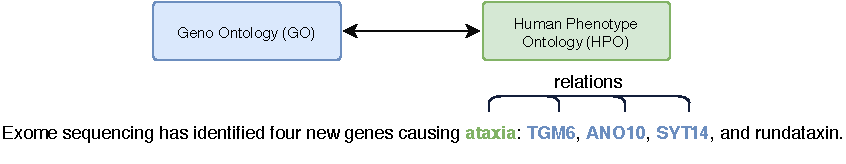
\includegraphics[width=15cm]{images/figure_example_pgr.pdf}
\caption[Example Sentence Presenting Human Phenotype-Gene Relations]{Example sentence describing three relations between the phenotype \textit{ataxia} and the genes \textit{TGM6}, \textit{ANO10}, and \textit{SYT14}, respectively. All entities can be linked to concepts in the HPO \citep{kohler2017human} (\textit{ataxia}) and GO \citep{ashburner2000gene} (\textit{TGM6}, \textit{ANO10}, and \textit{SYT14}) ontologies.} \label{fig3}
\end{figure}

The first release of the  PGR dataset focused mostly on the initial release of the dataset (10/12/2018), where a small subset of relations (6\%) was manually reviewed to evaluate the PGR dataset quality and also to use as test corpus for machine learning model evaluation. The second release (11/03/2019) captured a more clear-cut search of the type of abstracts to retrieve, such as abstracts regarding diseases, their associated phenotypes and genes, increasing from about 2.5 relations per abstract to about 3.0 relations per abstract, and the overall number of relations by 2-fold. 

The relations identified in the PGR dataset are either Known if present in the knowledge base of relations provided by the Human Phenotype Ontology (HPO) group \citep{kohler2017human} or Unknown otherwise. Table \ref{tab1} presents the numbers for the second release of the PGR dataset.


\begin{table}
\renewcommand\arraystretch{1.3}
\centering
\caption[Counts for the PGR Dataset]{The number of abstracts, phenotype and gene annotations, and of known, unknown and total of relations for the second release (11/03/2019) of the PGR dataset (partial table from \citep{sousa2019silver}).}\label{tab1}
\newcolumntype{A}{ >{\centering\arraybackslash} m{1.8cm} }
\begin{tabular}{|A|A|A|A|A|A|}
\hline
\multirow{2}{*}{\textbf{Abstracts}} & \multicolumn{2}{c|}{\textbf{Annotations}} & \multicolumn{3}{c|}{\textbf{Relations}} \\
\cline{2-6}
& \textbf{Phenotype} & \textbf{Gene} & \textbf{Known} & \textbf{Unknown} & \textbf{Total} \\
\Xhline{2\arrayrulewidth}
2657 & 9553 & 23786 & 2480 & 5483 & 7963 \\
\hline
\end{tabular}
\end{table}